\documentclass[12pt]{article}

\usepackage{theorem,amsmath,amssymb}
\usepackage{graphicx}


\addtolength{\topmargin}{-23mm}
\addtolength{\textheight}{60mm}
\addtolength{\oddsidemargin}{-20mm}
\addtolength{\textwidth}{40mm}

\def\eqref#1{(\ref{#1})}
\newcommand{\goth}{\mathfrak}
\newcommand{\arrow}{{\:\longrightarrow\:}}
\def\1{\sqrt{-1}\:}
\newcommand{\restrict}[1]{{\left|_{{\phantom{|}\!\!}_{#1}}\right.}}

\renewcommand{\bar}{\overline}
\renewcommand{\phi}{\varphi}
\renewcommand{\epsilon}{\varepsilon}
\renewcommand{\geq}{\geqslant}
\renewcommand{\leq}{\leqslant}

\def\rad{\operatorname{\sf rad}}
\def\tr{\operatorname{\sf tr}}
\def\rk{\operatorname{\sf rk}}
\def\Alt{\operatorname{\sf Alt}}
\def\Sym{\operatorname{\sf Sym}}
\def\Id{\operatorname{\sf Id}}
\def\Hom{\operatorname{Hom}}
\def\Map{\operatorname{Map}}
\def\Gal{\operatorname{Gal}}
\def\Aut{\operatorname{Aut}}
\newcommand{\End}{\operatorname{End}}
\newcommand{\Mat}{\operatorname{Mat}}

\newcommand{\coker}{\operatorname{Coker}}

\def\chpoly{\operatorname{\sf Chpoly}}
\def\minpoly{\operatorname{\sf Minpoly}}

\def\cchar{\operatorname{\sf char}}

\def\Z{{\mathbb Z}}
\def\R{{\mathbb R}}
\def\C{{\mathbb C}}
\def\Q{{\mathbb Q}}
\def\N{{\mathbb N}}
\def\F{{\mathbb F}}

\def\Re{\operatorname{Re}}
\def\Im{\operatorname{Im}}

\makeatletter
\theoremstyle{definition}

\newtheorem{zadacha}{������}[section]
\newtheorem{opredelenie}{�����������}[section]
\newtheorem*{ukazanie}{��������}%[section]
\newtheorem*{zamechanie}{���������}%[section]

%\renewcommand{\labelenumi}{\ralph{enumi}.}
\renewcommand{\labelenumi}{\alph{enumi}.}
\newcommand{\subs}[1]{{\bigskip\centerline{\bf\large #1}\bigskip}}
\newcommand{\sttr}{{\bf(*)}}
\newcommand{\shrk}{{\bf(!)}}
\newcommand{\doublesttr}{{\bf(**)}}

\newcommand{\listok}[2]{%
\setcounter{page}{1}
\renewcommand{\@oddhead}{\hfil #2 \hfil}
\renewcommand{\@evenhead}{\hfil #2 \hfil}
\section*{#2}
\refstepcounter{section}
\setcounter{section}{#1}
}

\@addtoreset{equation}{section}
\renewcommand{\theequation}{\thesection.\arabic{equation}}

\let\oldllim=\lim
\def\lim{\oldllim\limits}
\makeatother


\begin{document}

\listok{10}{Geometry 10: The fundamental group and the loop space}

%%%%%%%%%%%%%%%%%%%%%%%%%%%%%%%%%%%%%%%%%%%%%%%%%%%%%%%%%%%%

%%%%%%%%%%%%%%%%%%%%%%%%%%%%%%%%%%%%%%%%%%%%%%%%
\subs{Path-connectedness}
%%%%%%%%%%%%%%%%%%%%%%%%%%%%%%%%%%%%%%%%%%%%%%%%
\newcommand{\ts}{topological space}
\newcommand{\pc}{path-connected}
\begin{opredelenie}
Let $M$ be a \ts . Recall that a {\bf path} in  $M$ is 
a continuous mapping $[a, b] \stackrel \phi \arrow M$.
In this case one says that the path 
$\phi$ {\bf connects the points $\phi(a)$ and $\phi(b)$}.
$M$ is called {\bf \pc} when any two points
of $M$ can be connected by a path $[a, b] \stackrel \phi \arrow M$.
\end{opredelenie}

\begin{zadacha}
Let $a$, $b$, $c$ are points in  $M$, so that
$a$ can be connected (by a path) to $b$, and $b$ can be connected to $c$.
Show that $a$ can be connected to $c$.
\end{zadacha}

\begin{zadacha} 
From this derive that a union of \pc\ subsets of 
$M$ containing a point $x\in M$ is \pc .
\end{zadacha}

\begin{opredelenie}
The union of all the subsets of $M$, containing a fixed point
$x$ is called a {\bf \pc\ component} of $M$
\end{opredelenie}

\begin{zadacha} 
Consider $X\subset \R^2$ that is 
the union of the graph of the function  $\sin(1/t)$ and the segment
$[(0,1), (0,-1)]$. Show that $X$ is locally compact, connected, but not
\pc . Find its \pc\ components. 
\end{zadacha}

\begin{zadacha}[*]
Construct a compact, connected metrizable \ts\ with 
infinitely many \pc\ components.
\end{zadacha}

\begin{opredelenie}
Let $\{M_\alpha\}$ be a collection of \ts s 
indexed by the set ${\mathfrak A}$. The disjoint union
$\coprod_{\alpha \in \mathfrak A} M_\alpha$ is a \ts\ 
whose points are pairs 
$(\alpha,m) \ \ | \ \  \alpha\in {\mathfrak A}, m\in M_\alpha$,
and a base of the topology is given by the open sets in all
$M_\alpha$.
\end{opredelenie}

\begin{zadacha}
Show that the disjoint union of one-point spaces is discrete.
Show that the natural projection
$\coprod_{\alpha \in \mathfrak A} M_\alpha \arrow {\mathfrak A}$
on 
${\mathfrak A}$ with discrete topology is 
continuous.
\end{zadacha}


\begin{opredelenie}
A \ts\ $M$ is called locally connected (respectively, locally \pc ), 
if any point $x\in M$ is contained in a connected
(respectively, \pc ) open set.
\end{opredelenie}

\begin{zadacha} 
Let 
$M$ be a \ts . Show that $M$ is locally connected
(resp. locally \pc ) iff
$M$ is a disjoint union of its (path-)connected components.
\end{zadacha}

\begin{zadacha}
Show that a connected space is \pc\ iff it is locally \pc .
\end{zadacha}

\begin{zadacha}
Show that an open subset of $\R^n$ is locally \pc . 
\end{zadacha}

\begin{zadacha}[**]
Let $\omega$ be the smallest uncountable ordinal, and
$\phi:\; [0,1] \arrow \omega$ the corresponding bijection.
Let $X \subset [0,1]\times [0,1]$ be the subset of the square
constisting of $x,y$ satisfying $\phi(x) > \phi(y)$.
Show that $X$ is connected.  Show that \pc\ components of  
$X$ are either points or segments of horisontal intervals.
\end{zadacha}

\begin{ukazanie} 
Show that the intersection of 
$X$ with any vertical segment is nowhere dense.
Let $V\subset [0,1]\times [0,1]$ be a connected closed subset of the
square contained in 
$X$. Show that $V$ intersects each vertial segment in no more than 1 point.
Thus $V$ is the graph of a continuous mapping
$\gamma:\; [a,b] \arrow [0,1]$, satisfying
$\phi(\gamma(a))< \phi(a)$. Show that this mapping is constant.
\end{ukazanie}

%%%%%%%%%%%%%%%%%%%%%%%%%%%%%%%%%%%%%%%%%%%%%%%%
\subs{Geodesic connectedness}
%%%%%%%%%%%%%%%%%%%%%%%%%%%%%%%%%%%%%%%%%%%%%%%%

\begin{opredelenie}
Let $M$ be a complete locally compact metric space.
Recall that a {\bf geodesic} in 
$M$ is a metric-preserving mapping
$[a, b] \arrow M$.
We say that $M$ is {\bf geodesically connected} if any
two points can be connected by a geodesic.
Obviously such a space is \pc .
\end{opredelenie}

\begin{opredelenie}
Let $M$ be a complete locally compact metric space.
We say that $M$ is 
{\bf Lipschitz connected}, with Lipschitz constant
$C\geq 1$, if for any 
$x, y \in M$ and any $\epsilon >0$ there exists 
a sequence of points 
$x=x_1, x_2,\dots, x_n=y$ such that 
$d(x_i, x_{i+1})< \epsilon$, 
$\sum_i d(x_i, x_{i+1}) \leq C d(x,y)$.
In other words, one can place 
$n$ points between $x$ and $y$  so that they are at distance
at most
$\epsilon$ from each other, whereas the length of the polygonal line
they form is at most  $C d(x,y)$.
\end{opredelenie}

\begin{zadacha}[*] 
Show that any geodesically connected metric space
is Lipschitz connected with Lipschitz constant $1$.
\end{zadacha}

\begin{ukazanie}
This is Hopf-Rinow Theorem.
\end{ukazanie}

\begin{zadacha}[!] 
Let $(M, d)$  be a Lipshitz connected metric space, with constant $C$.
Define a function $d_h:\; M\times M \arrow \R$  as 
\[
\lim\limits_{\epsilon\arrow 0} \inf\left(\sum d(x_i, x_{i+1})\right),
\]
where $\inf$  is taken over such sequences 
$x=x_1, x_2, \dots, x_n=y$ that  $d(x_i, x_{i+1})< \epsilon$.
Show that 
$d(x, y) \leq d_h(x,y) \leq Cd(x,y)$
for any 
$x, y \in M$. Show that $d_h$ is a metric and that 
$(M, d)$ is homeomorphic to 
$(M, d_h)$.
\end{zadacha}

\begin{zadacha}[*]
Show that $(M, d_h)$ is Lipschitz connected, for any $C>1$. 
\end{zadacha}

\begin{zadacha}[*]
Show that $(M, d_h)$ satisfies Hopf-Rinow condition (and is therefore
geodesically connected).
\end{zadacha}

\begin{opredelenie}
Recall that a mapping $[a,b]\stackrel\phi\arrow M$ 
{\bf satisfies the Lipschitz condition, with constant 
$C>0$},
if $d(\phi(x),\phi(y)) \leq C|x-y|$ for any 
$x, y\in [a,b]$. It is easy to see that a Lipshitz mapping is
continuous.
\end{opredelenie}

\begin{zadacha}[*]
Let $M$ be a complete 
locally compact metric space.
Show that $M$ is Lipschitz connected with constant $C$ iff
one can connect any two points by a Lipschitz path with the
same (universal for $M$) constant.
\end{zadacha}

\begin{ukazanie} 
Use the previous problem and the inequality
$d(x, y) \leq d_h(x,y) \leq Cd(x,y)$.
\end{ukazanie}

\begin{zamechanie}
We have established that a Lipschitz connected metric space is 
\pc .
\end{zamechanie}

\begin{zadacha}  
Consider the circle $S$ on the plane with induced metric.
Show that $S$ is Lipschitz connected with constant
$\frac \pi 2$.
\end{zadacha}

\begin{zadacha}[*]
Show that $\frac \pi 2$ is the smallest possible constant
for which the circle with such a metric is Lipschitz connected.
\end{zadacha}

\begin{zadacha}[**]
Consider the mapping
$]0, \infty[ \arrow \R^2$,
given in polar coordinates by the function
$\theta = 1/x$, $r=x$ (this is a spiral winding around 0 
with the step $\frac 1 {2\pi n}$).
Let $X$ be the closure of the graph of this function
(that obviously consists of the graph itself and 0).
Show that $X$ is \pc . Show that
$X$ is not Lipschitz connected, no matter what constant $C$ we take.
\end{zadacha}

\begin{zadacha}[*]
Let $M$ be a locally compact complete metric space.
Denote by 
$S_\epsilon(x)$ the sphere of radius $\epsilon$ with the centre in $x$.
Show that the following conditions are equivalent.
\begin{enumerate}
\renewcommand{\labelenumi}{(\roman{enumi})}
\item $M$ is Lipschitz connected, with constant $C$

\item for any 
$x, y \in M$ and any $r_1, r_2 >0$ satisfying $r_1 + r_2 \leq 1$,
the distance between 
$S_{dr_1}(x)$ and $S_{dr_2}(y)$ is not bigger than 
$C d (1 - r_1 - r_2)$, where $d= d(x,y)$.
\end{enumerate}
\end{zadacha}


\begin{ukazanie}
To derive (ii) from Lipschitz connectedness, 
consider a Lipschitz curve through $x, y$.
Lipschitz connectedness follows immediately from (ii).
The distance from $x$ to  $S_{d(1-C^{-1}\epsilon)}(y)$
is at most $\epsilon$; take as  $x_2$
the point of the sphere realizing this distance
(that is possible, as the sphere is compact by Hopf-Rinow Theorem),
and use induction.
\end{ukazanie}

\begin{zamechanie}
Recall that in one version that Hopf-Rinow condition
says that the distance between  
$S_{dr_1}(x)$ and $S_{dr_2}(y)$
equals $d(1 - r_1 - r_2)$.  
\end{zamechanie}

%%%%%%%%%%%%%%%%%%%%%%%%%%%%%%%%%%%%%%%%%%%%%%%%%%%%%%%%%%%%
\subs{Loop space}
%%%%%%%%%%%%%%%%%%%%%%%%%%%%%%%%%%%%%%%%%%%%%%%%%%%%%%%%%%%%

\begin{opredelenie}
Let $(M, x)$ be a topological space with a marked point $x$.
Consider the set $\Omega(M, x)$ of paths 
$[0, 1] \stackrel \phi \arrow M$, $\phi(0) = \phi(1) = x$,
with open-compact topology (the base of this topology consists of 
the set $U(K, W)$ of mappings of a given compact
$K\subset [0,1]$ into a given open set $W\subset M$). 
The $\Omega(M, x)$ is called 
{\bf the loop space} for $(M,x)$.
\end{opredelenie}

\begin{zadacha}[!]
Let $M$ be metrizable. Show that
$\Omega(M, x)$ is metrizable too, with the metric
\[ d(\gamma, \gamma') = \sup_{x\in[0,1]}d(\gamma(x),
\gamma'(x)).
\]
\end{zadacha}

\begin{zadacha}
Let $(M, x)$ be a space with a marked point $x$.
$M_0$ the connected component of $x$, and $M_1$ the \pc\ 
component of $x$. Show that
$\Omega(M, x)=\Omega(M_0, x)=\Omega(M_1, x)$.
\end{zadacha}

\begin{zadacha}
Let $X, Y$ be compacts, $\cal W$ be the space of mappings from  
$X$ to  $M$ endowed with open-compact topology.
Construct a bijection between continuous mappings
from  $Y$ to $\cal W$ and continuous mappings
$X \times Y \arrow M$.
\end{zadacha}


\begin{zadacha}[!]
Let $\gamma, \gamma'\in \Omega(M,x)$. Construct a bijection between the
following sets:
\begin{enumerate}
\renewcommand{\labelenumi}{(\roman{enumi})}
\item Paths $\Gamma:\; [0, 1] \arrow \Omega(M,x)$,
connecting $\gamma$ and $\gamma'$.

\item Continuous mappings $\Psi$ from the square
$[0,1]\times [0,1]$ to $M$ that map $\{1\}\times [0,1]$
to $x$ and such that 
$\Psi\restrict{[0,1]\times \{0\}} = \gamma$,
$\Psi\restrict{[0,1]\times \{1\}} = \gamma'$.
\end{enumerate}
\end{zadacha}

\begin{opredelenie}
Paths $\gamma, \gamma'\in \Omega(M,x)$ for which
the mappings
$\Psi:\; [0,1]\times [0,1]\arrow M$ exist, are called 
{\bf homotopic}, and $\Psi$, that connectes them, is called 
{\bf homotopy}.
\end{opredelenie}

\begin{zadacha} 
Show that the set of loops homotopic to 
$\gamma\in \Omega(M,x)$ is a \pc\  component of
$\gamma\in \Omega(M,x)$.
\end{zadacha}

\begin{zadacha}
Show that the homotopy of loops is an equivalence relation.
\end{zadacha}

\begin{zamechanie} 
Loops homotopic to each other are also called {\bf homotopy equivalent}.
\end{zamechanie}

\begin{opredelenie}
Let $(M, x)$ be \pc . The set of homotopy equivalent classes of loops is
denoted by $\pi_1(M, x)$.
\end{opredelenie}

\begin{zadacha}[*]
Let $M\subset \R^2$ be the union of the closed segment 
$[(0,1), (0,-1)]$ and arcs of circles of diameters
$3, 4, 5, \dots$ that connect  $(0,1)$ and $(0,-1)$.
\begin{center}
%
\epsfig{file=geom10b.eps,width=0.5\linewidth}

\includegraphics[height=40mm]{geom10b}
\end{center}
Show that $M$ is \pc .  Show that for any $x\in M$ the space 
$\Omega(M,x)$ is not locally \pc .
\end{zadacha}

\begin{zadacha}[*] \label{_edi_geode_Zadacha_}
Let $(M,d)$ be a geodesically connected 
locally compact metric space such that  for a
$\delta >0$ and any
$x, y\in M$, $d(x,y)<\delta$, the geodesic connecting
$x$ and $y$ is unique. Let
$\Delta_\delta\subset M\times M$ be the set of pairs 
$x, y\in M$, $d(x,y)<\delta$. Consider the mapping
$\Delta_\delta\arrow M$ of pairs to the middle points of
the geodesics that connect pairs. Show that it is continuous.
\end{zadacha}

\begin{ukazanie}
Let $\{(x_i, y_i)\}$ is a sequence of pairs converging to 
$(x,y)$, and 
$\{z_i\}$ the sequence of middle points of corresponding geodesics.
Due to local compactness, $\{z_i\}$ has limit points and does not
contain infinite discrete subsets. Any limit point of
$\{z_i\}$ will be the middle of geodesic connecting
$x$ and $y$. Thus
$\{z_i\}$ has unique limit point.
\end{ukazanie}

\begin{zadacha}[*]
Consider the mapping
$\Delta_\delta\otimes [0,1] \stackrel \Psi \arrow M$, 
of pairs $x, y\in M$, $d(x,y)=d$, 
� $t\in [0,1]$ to points
$\gamma_{x,y}\left(\frac t d\right)$, where
$\gamma_{x,y}$ is a geodesic connecting
$x$ and $y$ (when $x=y$ set
$\Psi(x,y,t)=x$). Show that this mapping is continuous.
\end{zadacha}

\begin{ukazanie}
Use the previous problem and the construction of a geodesic as the
limit of middle points of segments used in the proof of Hopf-Rinow
Theorem.
\end{ukazanie}

\begin{opredelenie}
Let $M$ be a metric space. A path
$\gamma:\; [0,1] \arrow M$  is called {\bf piecewise geodesic}
if $[0,1]$ is subdivided into
$[0, a_1]$, $[a_1, a_2]$, $\ldots$, $[a_n, 1]$,
and on each of these closed intervals
$\gamma$ satisfies
$d (\gamma(x), \gamma(y)) = \lambda_i|x-y|$,
for some constant $\lambda_i$
\end{opredelenie}

\begin{zamechanie}
If $M$ is an open set in  $\R^n$ with the natural metric
then, as shown is Sheet 4, geodesics are segments.
Thus piecewise geodesics are piecewise linear.
Such mappings are also called {\bf piecewise linear}.
\end{zamechanie}

\begin{zadacha}[*]
In the conditions of Excercise~\ref{_edi_geode_Zadacha_}, consider
$\Omega(M,x)$ as a metric space (with $\sup$-metric). 
Show that any loop $\gamma\in\Omega(M,x)$ is homotopic to 
a piecewise geodesic, so that the homotopy can be chosen in any
$\epsilon$-neighbourhood $B_\epsilon(\gamma)\subset \Omega(M,x)$.
\end{zadacha}

\begin{zadacha}[*]
Derive from this that
$\Omega(M,x)$ is locally \pc .
\end{zadacha}

\begin{zamechanie}
In this case $\pi_1(M, x)$ is the set of connected
components of $\Omega(M, x)$.
\end{zamechanie}

\begin{zadacha} 
Let $M$ be an open set in $\R^n$. Show that
$\Omega(M, x)$ is locally \pc .
\end{zadacha}

\begin{ukazanie}
Show that any loop can be homotopically deformed, in a
sufficiently small $\epsilon$-neighbourhood, into a piecewise linear.
\end{ukazanie}

%%%%%%%%%%%%%%%%%%%%%%%%%%%%%%%%%%%%%%%%%%%%%%%%
\subs{Fundamental group}
%%%%%%%%%%%%%%%%%%%%%%%%%%%%%%%%%%%%%%%%%%%%%%%%

\begin{zadacha}\label{_proizvede_Zadacha_}
Given loops  $\gamma_1, \gamma_2 \in \Omega(M, x)$,
consider the loop $\gamma_1 \gamma_2\in \Omega(M, x)$, 
defined as follows:
\[
\gamma_1 \gamma_2(\lambda) = 
\begin{cases}
\gamma_1(2\lambda) &\qquad \lambda\in [0, 1/2],\\
\gamma_2(2\lambda-1) &\qquad \lambda\in [1/2,1].
\end{cases}
\]
Show that the class of the homotopy $\gamma_1\gamma_2$ depends only
on classes of homotopies 
$\gamma_1$, $\gamma_2$: if
$\gamma_1\sim\gamma_1'$, $\gamma_2\sim\gamma_2'$
then $\gamma_1\gamma_1'\sim \gamma_2\gamma_2'$.
\end{zadacha}

\begin{zadacha}
Show that $(\gamma_1\gamma_2)\gamma_3$ is homotopy equivalent to 
$\gamma_1 (\gamma_2\gamma_3)$.
\end{zadacha}

\begin{zadacha} 
Given a loop $\gamma \in \Omega(M, x)$, denote by 
$\gamma^{-1}$ the loop $\gamma^{-1}(x) = \gamma(1-x)$. Show that the
loops $\gamma \gamma^{-1}$ and $\gamma^{-1} \gamma$ are homotopic to the
trivial loop $[0,1]\arrow x$.
\end{zadacha}

\begin{zamechanie}
Loops that are homotopic to the trivial one are called {\bf null-homotopic}.
\end{zamechanie}

\begin{zadacha}[!]
Show that the operation $\gamma_1, \gamma_2\arrow \gamma_1\gamma_2$
makes  $\pi_1(M, x)$  into a group.
\end{zadacha}

\begin{opredelenie} 
This group is called {\bf the fundamental group} of $M$.
\end{opredelenie}

\begin{zadacha}
Let $X\stackrel f \arrow Y$ be a continuous mapping of \pc\ spaces,
and $x\in X$. Consider the corresponding mapping
$$
\Omega(X, x) \overset{\check{f}}{\arrow} \Omega(Y, f(y)),
\qquad \gamma \mapsto \gamma\circ f.
$$
Show that $\check f$ maps homotopic paths to homotopic and
induces a homomorphism of fundamental groups.
\end{zadacha}

\begin{zadacha}
Let $M$ be a \pc\ topological space, 
and $x, y \in M$. Consider the space
$\Omega(M, x, y)$ of paths
$[0,1]\arrow M$ connecting
$x$ and $y$ with open-compact topology.
As above, paths are called homotopic (homotopy equivalent)
is they lie in the same \pc\ component
of $\Omega(M, x, y)$. Define an operation
$\Omega(M, x, y) \times \Omega(M, y, z)\arrow \Omega(M,x, z)$,
$\gamma_1, \gamma_2 \mapsto \gamma_1\gamma_2$
using the same formula as in Excercise~\ref{_proizvede_Zadacha_}. 
Show that this mapping is continuous and maps homotopic paths
to homotopic.
\end{zadacha}

\begin{zadacha}[!]
Let $x, y \in M$, and $\gamma_{xy}[0,1] \arrow M$ be a path connecting 
$x$ and $y$. Define
$\gamma_{xy}^{-1}$ using 
$\gamma_{xy}^{-1}(\lambda) = \gamma_{xy}(1-\lambda).$
Consider the mapping $\Omega(M,x) \arrow \Omega(M, y)$, 
$\gamma \mapsto \gamma_{xy}^{-1}\gamma \gamma_{xy}$
and $\Omega(M,y) \arrow \Omega(M, x)$, 
$\gamma \mapsto \gamma_{xy}\gamma \gamma_{xy}^{-1}$.
Show that these mappings map homotopic paths to homotopic. 
Let $f$, $g$ be corresponding maps on fundamental groups.
Show that $f$ � $g$ are inverses of each other and induce
an isomorphism of groups
$\pi_1(M, x)\stackrel{\phi_{\gamma_{xy}}}\arrow \pi_1(M, y)$.
\end{zadacha}

\begin{zamechanie}
As can be seen from the preceding problem, if 
$\pi_1(M)$ is not abelian then the isomorphism 
$\pi_1(M, x)\cong \pi_1(M, y)$
obtained there nontrivially
depends upon the  choice of the path  
$\gamma_{xy}$. Nevertheless, when the dependence upon the
marked point is not important, the fundamental group
$M$ is denoted simply by $\pi_1(M)$. This notation is not quite correct.
\end{zamechanie}

\begin{zadacha}[!]
In conditions of the preceding problem, let 
$x=y$, and  $\gamma_{xx}$ a path. Show that the isomorphism
$\pi_1(M, x)\stackrel{\phi_{\gamma_{xx}}}\arrow \pi_1(M, x)$
obtained above
can be expressed via $\gamma_{xx}$  as follows:
$\gamma \arrow \gamma_{xx} \gamma \gamma_{xx}^{-1}$.
\end{zadacha}

%%%%%%%%%%%%%%%%%%%%%%%%%%%%%%%%%%%%%%%%%%%%%%%%
\subs{Simply connected spaces}
%%%%%%%%%%%%%%%%%%%%%%%%%%%%%%%%%%%%%%%%%%%%%%%%


\begin{opredelenie}
Let $M$ be a \pc\ topological space.
We say that
$M$ is {\bf simply connected} when all the loops on $M$
are contractible, i.e. when
$\pi_1(M) = \{1\}$.
\end{opredelenie}

\begin{zadacha} Show that $\R^n$ is simply connected. 
\end{zadacha}

\begin{opredelenie}
Let $(M, x)$ be a topological space with a marked point,
$M \times [0,1] \stackrel \phi\arrow M$ be a continuous mapping
such that
$\phi(M\times \{1\}) = \{x\}$ and
$\phi \restrict{M\times \{0\}}$ the identity mapping
from $M= M\times \{0\}$ to $M$. Then $(M,x)$
is called {\bf contractible}.
In this case  one says that $\phi$ {\bf defines a homotopy between the
  identity mapping and the projection $M\arrow \{x\}$.}
\end{opredelenie}

\begin{zadacha}[!]
Let $(M, x)$ be \pc\  and contractible.
Show that for any point
$y\in M$ the space $(M, y)$ is contractible.
\end{zadacha}

\begin{ukazanie} 
Let $M \times [0,1] \stackrel \phi\arrow M$ be a homotopy between 
the identity mapping and the projection onto 
$\{x\}$, and  $[1,0]\stackrel\gamma\arrow M$ be a path connecting
$x$ and $y$. Take
$M \times [0,1] \overset{\phi_1}{\arrow} M$,
mapping $(m, t)$ to $\phi(m, 2t)$ for
$t\in [0,1/2]$ and $(m, t)$ in
$\gamma(2t-1)$ for $t\in [1/2,0]$.
\end{ukazanie}

\begin{zadacha}
Show that a contactible topological space is \pc .
\end{zadacha}

\begin{zamechanie} 
Two preceding problems immediately imply that
the contractibility of $(M, x)$ does not depend upon the choice of
$x$. Thus we say in the remainder simply 
``$M$ is contractible''.
\end{zamechanie}

\begin{zadacha} 
Show that a contractible space is simply connected.
\end{zadacha}

\begin{zadacha}[!]
Let $V\subset \R^n$ be a {\bf star subset} of
$(\R^n, x)$, that is, it satisfies the property that any line through
$x\in \R^n$ intersects $V$ in a connected set, and
$x\in V$. Show that $V$ is contractible.
\end{zadacha}

\begin{zadacha}
Let $V\subset \R^n$ be a convex set. Show that it is contractible.
\end{zadacha}

\begin{opredelenie}
Let $N$ be a subset of a toplogical space $M$.
The {\bf deformation retract}
(or simply {\bf retract}) of 
$M$ to  $N$ is a continuous mapping
$M \times [0,1] \stackrel \phi\arrow M$, such that
$\phi(M\times \{1\}) \subset N$, its restriction onto
$N$ the identity, and $\phi \restrict{M\times \{0\}}$ an identity mapping.
In this case $N$ is called a {\bf retract} of $M$.
\end{opredelenie}

\begin{zadacha}[!]
Let  $N$ be a retract of $M$, and $n\in N$.
Show that the natural mapping
$\pi_1(N, n)\arrow \pi_1(M, n)$ is an isomorphism. 
\end{zadacha}

\begin{opredelenie}
Let $M$ be a topological space,  and $\sim$ be an equivalence relation.
As always, the set of equivalence classes is denoted by  
$M/\sim$. 
We introduce on $M/\sim$ the {\bf quotient topology}:
the open subsets of $M/\sim$ are those, whose preimages in $M$ are open.  
In particular, if $G$ is a group acting on $M$, there is 
the natural (orbit) equivalence relation on $M$:
$x \sim y$ if there exists $g \in G$ satisfying $g \cdot x = y$.
The quotient of $M$ w.r.t. this equivalence relation
is called the quotient space w.r.t. the $G$-action and denoted by
$M/G$. The corresponding equivalence classes are called {\bf $G$-orbits}
of $M$.
\end{opredelenie}

\begin{zadacha}\label{_hausdo_kone_Zadacha_}
Let $M$ be a Hausdorff topological space and
$\{x_1, \dots, x_n\} \subset M$ and  $\{y_1, \dots, y_m\} \subset M$ 
two disjoint finite subsets. Show that for these subsets
there exist non-intersecting neighbourhoods.
\end{zadacha}

\begin{zadacha}[!]
Let $M$ be a Hausdorff topological space and
$G$ a finite group of $M$-homeo\-mor\-phisms.
Show that  $M/G$ is Hausdorff.
\end{zadacha}

\begin{ukazanie}
Let $x,y$ be two points in distinct $G$-orbits.
Find non-intersecting $G$-invariant neighbourhoods of $x$ and $y$.
For this, apply Excercise~\ref{_hausdo_kone_Zadacha_} to the orbits
$Gx$, $Gy$, obtain neighbourhoods $U$, $U'$,
and pick $\bigcap_{g\in G} gU$, $\bigcap_{g\in G} gU'$.
\end{ukazanie}

\begin{zadacha}[*]
Give an example of a Hausdorff space
$M$ and non-Hausdorff space $M/G$ (here the group $G$ will be infinite).
\end{zadacha}

\begin{opredelenie}
Let $\Gamma$ be a graph, that is, a data collection  consistiting of  
``vertex set'' $\{\cal V\}$ and 
``edge set'' $\{\cal R\}$, and information on which vertices are
endpoints of which edges.
\begin{center}
%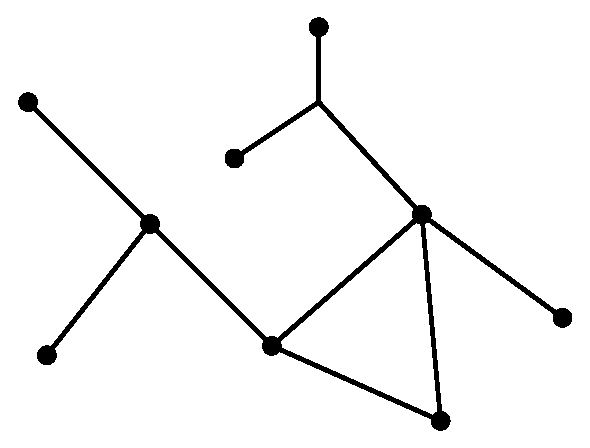
\epsfig{file=geom10a.eps,width=0.5\linewidth}
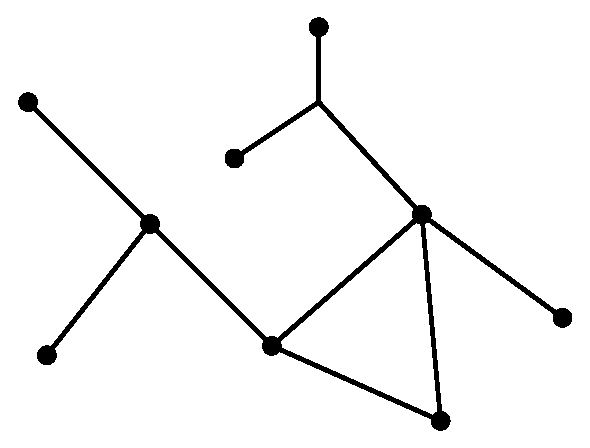
\includegraphics[height=60mm]{geom10a}
\end{center}
More precisely, one may define $\Gamma$ as a pair of sets
${\cal V}$, $\cal R$ and a surjection
$\{\cal R\}\times\{0,1\} \stackrel\Gamma\arrow \{\cal V\}$. 
Introduce on $\{\cal R\}\times [0,1]$ the equivalence relation 
generated by the following: endpoints of two edges are equivalent if
the are incident to the same vertex.
This relatin glues together endpoints of edges through the same vertex.
The quotient  $\{\cal R\}\times [0,1]$ w.r.t. this equivalence
relation is called the {\bf topological space of the graph}. 
\end{opredelenie}

\begin{zadacha}
Show that the topological space of any graph is Hausdorff.
\end{zadacha}

\begin{zadacha}
A graph is called connected if any vertex is connected to any other vertex
by a sequence of edges. Show that the topological space of a connected
graph is \pc .
\end{zadacha}

\begin{zadacha}[**]
Let $\Gamma$ be a graph with infinite vertex set.
Show that $\Gamma$ contains either an infinite clique
(i.e. the set of pairwise connected by edges vertices), or
an infinite coclique
(i.e. the set of vertices such that none of them are connected by
an edge).
\end{zadacha}

\begin{zadacha}[!]
Let $\Gamma$ be a connected graph with $n$ vertices and $n-1$ edges
(such a graph is called a {\bf tree}).  
\begin{center}
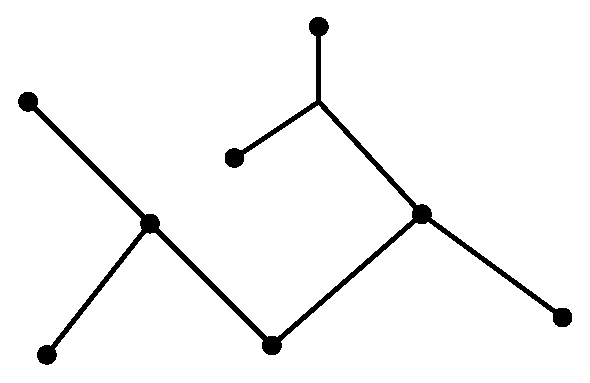
\includegraphics[height=40mm]{geom10c}
%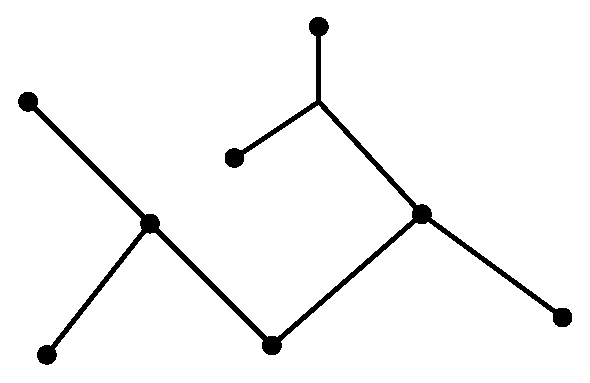
\epsfig{file=geom10c.eps,width=0.5\linewidth}
\end{center}
Show that the topological space $M_\Gamma$ of $\Gamma$ is contractible.
\end{zadacha}

\begin{zadacha}[*]
Let $\Gamma$ be an infinite graph so that each of its connected finite
subgraphs is a tree. Show that $\pi_1(M_\Gamma)=\{1\}$.
\end{zadacha}

\begin{zadacha}[*]
Let $S^n$ be an $n$-dimensional sphere ($n> 1$). Show that 
$S^n$ is simply connected.
\end{zadacha}

\begin{ukazanie}
Use geodesic connectedness.
\end{ukazanie}

%%%%%%%%%%%%%%%%%%%%%%%%%%%%%%%%%%%%%%%%%%%%%%%%
\subs{Coverings}
%%%%%%%%%%%%%%%%%%%%%%%%%%%%%%%%%%%%%%%%%%%%%%%%

\begin{opredelenie}
Let $\tilde M \stackrel \pi \arrow M$ be a continuous mapping of
topological spaces;
$\pi$ is called a {\bf covering} when any point has a neighbourhood
$U$ such that $\pi^{-1}(U)$ is the product of 
$U$ and a discrete topological space
$K$, so that the natural mapping
$\pi^{-1}(U)\stackrel \pi \arrow U$
coincided the projection
$\pi^{-1}(U) = U \times K \arrow U$.
In this case one also says that 
$\tilde M$ {\bf covers} $M$.
\end{opredelenie}

We consider the circle
$S^1$ as the quotient $S^1 = \R/\Z$.
This gives a natural group structure on $S^1$.

\begin{zadacha}
Let $n\neq 0$ be an integer. 
Condider a natural mapping 
$S^1 \arrow S^1$, $t \arrow nt$. Show that it is a covering.
\end{zadacha}

\begin{zadacha} 
Show that the natural projection
$\R \arrow  S^1 = \R/\Z$ is a covering.
\end{zadacha}

\begin{zadacha}
Show that the natural projection
$\R^n \arrow (S^1)^n$ is a covering.
\end{zadacha}

\begin{zadacha} 
Consider the quotient $S^n \arrow S^n/\{\pm 1\}= \R P^n$
of the sphere w.r.t. the central symmetry, with the natural topology.
Show that it is a covering.
\end{zadacha}

\begin{zadacha}
Let $\tilde M \stackrel \pi \arrow M$ be a covering, and  
$\tilde M'\subset M$ a subspace that covers $M$, too. Show that
$\tilde M'$ is clopen in $\tilde M$.
\end{zadacha}

\begin{zadacha}
Let $\tilde M \stackrel \pi \arrow M$ be a covering, and $M$ \pc . 
Show that 
$\tilde M$ is locally \pc . Show that any \pc\ component of 
$\tilde M$ covers $M$.
\end{zadacha}

\begin{zadacha}[!] \label{_nakry_line_svya_Zadacha_}
Let $\tilde M \stackrel \pi \arrow M$ 
be a covering, and $M$ \pc . Show that 
$\tilde M$ is connected iff it is \pc .
\end{zadacha}

\begin{opredelenie} 
Let $\gamma:\; [a, b] \arrow M$ be a path, and  
$\tilde M \stackrel \pi \arrow M$ a covering of  
$M$. A mapping
$\tilde \gamma:\; [a, b] \arrow \tilde M$
is called a {\bf lifting of $\gamma$} if
$\tilde \gamma\circ \pi = \gamma$.
\end{opredelenie}

\begin{zadacha}[!]
Let $\tilde M \stackrel \pi \arrow M$ be a covering,
and $\gamma:\; [a, b] \arrow M$ a path joining $x$ and $y$.
Show that for any $\tilde x\in \pi^{-1}(\{x\})$ the lifting
$\tilde \gamma$, mapping $a$ to $\tilde x$, exists, and is unique.
\end{zadacha}

\begin{zadacha}[!] \label{_konec_puti_Zadacha_}
Show that homotopic paths are lifted to homotopic paths, and that
$\tilde \gamma(y)\in \pi^{-1}(\{y\})$ is uniquely determined by the
class of the homotopy $\gamma$ in  
$\Omega(M, x, y)$ and the point $\tilde x$.
\end{zadacha}

\begin{zamechanie}
Denote by $\pi_1(M, x, y)$ the set of classes of homotopic paths from 
$x$ to $y$. We have a mapping 
\[ \pi^{-1}(\{x\})\times \pi_1(M, x, y) \stackrel \Psi\arrow \pi^{-1}(\{y\})
\]
\end{zamechanie}


\begin{opredelenie}
Let $\tilde M \stackrel \pi \arrow M$ be a cover, and $M$ \pc .
The space
$\tilde M$ is called a 
{\bf universal cover} if it is connected and simply connected.
\end{opredelenie}

\begin{zamechanie}
Simple connectedness was defined for \pc\ spaces only.
But this does not present an obstacle, as it follows from the
Excercise~\ref{_nakry_line_svya_Zadacha_} that
$\tilde M$ is \pc . 
\end{zamechanie}

\begin{zadacha}[!]
Let $\tilde M\stackrel \pi  \arrow M$ be a universal cover. 
Fix
$x\in M$ and $\tilde x\in \pi^{-1}(\{x\})$.
Consider the mapping
$\pi_1(M, x) \stackrel \psi \arrow \pi^{-1}(\{x\})$,
constructed in Excercise~\ref{_konec_puti_Zadacha_}, and
$\psi(\gamma) = \Psi(\tilde x, \gamma)$.
Show that it is a bijection.
\end{zadacha}

\begin{zadacha} 
Show that $\pi_1(S^1) = \Z$.
\end{zadacha}

\begin{zadacha} Show that $\pi_1((S^1)^n) = \Z^n$.
\end{zadacha}

\begin{zadacha}[*]
Show that for ($n>1$) one has $\pi_1(\R P^n)= \Z/2\Z$.
\end{zadacha}

\begin{zadacha}
Find the fundamental groups of all the  
letters of Greek alphabet,
except $\Phi$ and $B$. (More precisely, graphs modelled by these
letters.)
\end{zadacha}

\begin{zadacha}[*]
Given a finite connected graph with $n$ edges and $n$ vertices,
consider its topological space $M$.
Show that $\pi_1(M)=\Z$.
\end{zadacha}

\end{document}

